\documentclass[journal,12pt,twocolumn]{IEEEtran}
\usepackage{amsthm}
\allowbreak
\usepackage{setspace}
\usepackage{gensymb}
\singlespacing
\usepackage[cmex10]{amsmath}
\usepackage{caption}
\usepackage{amsthm}

\DeclareUnicodeCharacter{2212}{-}
\usepackage{tikz}
\usepackage{pgfplots}

\usepackage{mathrsfs}
\usepackage{txfonts}
\usepackage{stfloats}
\usepackage{bm}
\usepackage{cite}
\usepackage{cases}
\usepackage{subfig}

\usepackage{longtable}
\usepackage{multirow}

\usepackage{enumitem}
\usepackage{mathtools}
\usepackage{steinmetz}
\usepackage{tikz}
\usepackage{circuitikz}
\usepackage{verbatim}
\usepackage{tfrupee}
\usepackage[breaklinks=true]{hyperref}
\usepackage{graphicx}
\usepackage{tkz-euclide}
\graphicspath{ {./images/} }
\usetikzlibrary{calc,math}
\usepackage{listings}
    \usepackage{color}                                            %%
    \usepackage{array}                                            %%
    \usepackage{longtable}                                        %%
    \usepackage{calc}                                             %%
    \usepackage{multirow}                                         %%
    \usepackage{hhline}                                           %%
    \usepackage{ifthen}                                           %%
    \usepackage{lscape}     
\usepackage{multicol}
\usepackage{chngcntr}

\DeclareMathOperator*{\Res}{Res}

\renewcommand\thesection{\arabic{section}}
\renewcommand\thesubsection{\thesection.\arabic{subsection}}
\renewcommand\thesubsubsection{\thesubsection.\arabic{subsubsection}}

\renewcommand\thesectiondis{\arabic{section}}
\renewcommand\thesubsectiondis{\thesectiondis.\arabic{subsection}}
\renewcommand\thesubsubsectiondis{\thesubsectiondis.\arabic{subsubsection}}


\hyphenation{op-tical net-works semi-conduc-tor}
\def\inputGnumericTable{}                                 %%

\lstset{
%language=C,
frame=single, 
breaklines=true,
columns=fullflexible
}
\begin{document}


\newtheorem{theorem}{Theorem}[section]
\newtheorem{problem}{Problem}
\newtheorem{proposition}{Proposition}[section]
\newtheorem{lemma}{Lemma}[section]
\newtheorem{corollary}[theorem]{Corollary}
\newtheorem{example}{Example}[section]
\newtheorem{definition}[problem]{Definition}

\newcommand{\BEQA}{\begin{eqnarray}}
\newcommand{\EEQA}{\end{eqnarray}}
\newcommand{\define}{\stackrel{\triangle}{=}}
\bibliographystyle{IEEEtran}
\raggedbottom
\setlength{\parindent}{0pt}
\providecommand{\mbf}{\mathbf}
\providecommand{\pr}[1]{\ensuremath{\Pr\left(#1\right)}}
\providecommand{\qfunc}[1]{\ensuremath{Q\left(#1\right)}}
\providecommand{\sbrak}[1]{\ensuremath{{}\left[#1\right]}}
\providecommand{\lsbrak}[1]{\ensuremath{{}\left[#1\right.}}
\providecommand{\rsbrak}[1]{\ensuremath{{}\left.#1\right]}}
\providecommand{\brak}[1]{\ensuremath{\left(#1\right)}}
\providecommand{\lbrak}[1]{\ensuremath{\left(#1\right.}}
\providecommand{\rbrak}[1]{\ensuremath{\left.#1\right)}}
\providecommand{\cbrak}[1]{\ensuremath{\left\{#1\right\}}}
\providecommand{\lcbrak}[1]{\ensuremath{\left\{#1\right.}}
\providecommand{\rcbrak}[1]{\ensuremath{\left.#1\right\}}}
\theoremstyle{remark}
\newtheorem{rem}{Remark}
\newcommand{\sgn}{\mathop{\mathrm{sgn}}}
\providecommand{\abs}[1]{$\left\vert#1\right\vert$}
\providecommand{\res}[1]{\Res\displaylimits_{#1}} 
\providecommand{\norm}[1]{$\left\lVert#1\right\rVert$}
%\providecommand{\norm}[1]{\lVert#1\rVert}
\providecommand{\mtx}[1]{\mathbf{#1}}
\providecommand{\mean}[1]{E$\left[ #1 \right]$}
\providecommand{\fourier}{\overset{\mathcal{F}}{ \rightleftharpoons}}
%\providecommand{\hilbert}{\overset{\mathcal{H}}{ \rightleftharpoons}}
\providecommand{\system}{\overset{\mathcal{H}}{ \longleftrightarrow}}
	%\newcommand{\solution}[2]{\textbf{Solution:}{#1}}
\newcommand{\solution}{\noindent \textbf{Solution: }}
\newcommand{\cosec}{\,\text{cosec}\,}
\providecommand{\dec}[2]{\ensuremath{\overset{#1}{\underset{#2}{\gtrless}}}}
\newcommand{\myvec}[1]{\ensuremath{\begin{pmatrix}#1\end{pmatrix}}}
\newcommand{\mydet}[1]{\ensuremath{\begin{vmatrix}#1\end{vmatrix}}}
\numberwithin{equation}{subsection}
\makeatletter
\@addtoreset{figure}{problem}
\makeatother
\let\StandardTheFigure\thefigure
\let\vec\mathbf
\renewcommand{\thefigure}{\theproblem}
\def\putbox#1#2#3{\makebox[0in][l]{\makebox[#1][l]{}\raisebox{\baselineskip}[0in][0in]{\raisebox{#2}[0in][0in]{#3}}}}
     \def\rightbox#1{\makebox[0in][r]{#1}}
     \def\centbox#1{\makebox[0in]{#1}}
     \def\topbox#1{\raisebox{-\baselineskip}[0in][0in]{#1}}
     \def\midbox#1{\raisebox{-0.5\baselineskip}[0in][0in]{#1}}
\vspace{3cm}
\title{AI1103: Assignment 4}
\author{Tanmay Garg \\CS20BTECH11063 EE20BTECH11048}
\maketitle
\newpage
\bigskip
\renewcommand{\thefigure}{\theenumi}
\renewcommand{\thetable}{\theenumi}
Download all python codes from 
\begin{lstlisting}
https://github.com/tanmaygar/AI-Course/blob/main/Assignment4/codes/GATE-2015(CS-SET-3)-Q37.py
\end{lstlisting}
%
and latex-tikz codes from 
%
\begin{lstlisting}
https://github.com/tanmaygar/AI-Course/blob/main/Assignment4/Assignment4.tex
\end{lstlisting}
\section*{Problem GATE 2015(CS-SET 3), Q.37: }
Suppose $X_i$ for $i = 1, 2, 3$ are independent
and identically distributed random variables
whose probability mass functions are
$\pr{X_i = 0} = \pr{X_i = 1} = \frac{1}{2}$ for $i = 1, 2, 3$.
Define another random variable $Y = X_1 X_2 \oplus X_3$, where $\oplus$ denotes XOR. Then $\pr{Y = 0|X_3 = 0} =$

\section*{Solution:}
We know that
\begin{align}
    \pr{Y=0|X_3=0} &= \dfrac{\pr{Y=0,X_3=0}}{\pr{X_3=0}} \label{eq:0.0.1}\\
    \pr{X_3 = 0} &= \frac{1}{2} \label{eq:0.0.2}
\end{align}
For
\begin{align}
    Y &= 0\\
    X_1X_2 \oplus X_3 &= 0\\
    \because X_3 = 0,\quad \therefore X_1X_2 &= 0
\end{align}
%The number of possibilities for $X_1X_2=0$
%\begin{align}
%    (X_1,X_2) = \begin{cases}
%(0,0)\\(0,1)\\(1,0)
%\end{cases}
%\end{align}

Since the random variables are independent of each other
\begin{align}
    \pr{X_i = a, X_j = b} &= \pr{X_i=a} \cdot \pr{X_j=b}\\
    i &\neq j\\
    a,b &\in \{0,1\}\\
    i,j &\in \{1,2,3\}
\end{align}
\begin{table}[h!]
    \centering
    \resizebox{\columnwidth}{!}
    {
    \begin{tabular}{|c|c|c|}
    \hline
         $\pr{X_1=0,X_2=0}$& $\pr{X_1=0}\cdot\pr{X_2=0}$&$0.25 $\\ \hline
         
         $\pr{X_1=1,X_2=0}$&$\pr{X_1=1}\cdot\pr{X_2=0}$&$0.25$ \\  \hline
         $\pr{X_1=0,X_2=1}$&$\pr{X_1=0}\cdot\pr{X_2=1}$&$0.25$\\
         \hline
    \end{tabular}
    }
    
    \caption{Probabilities }
    \label{tab:my_label}
\end{table}
\begin{align}
\nonumber
\pr{X_1X_2=0} &= \pr{X_1=0,X_2=0} \\ \nonumber
    &\quad+ \pr{X_1=0,X_2=1}\\ &\quad+ \pr{X_1=1,X_2=0}\\
    &=\frac{1}{4} +\frac{1}{4} + \frac{1}{4}= \frac{3}{4} 
\end{align}
\begin{align}
    \pr{Y=0,X_3=0} &= \pr{X_1X_2=0}\cdot\pr{X_3=0}\\
    &=\frac{3}{4} \cdot \frac{1}{2}\\
    &=\frac{3}{8} \label{eq:0.0.15}
\end{align}
Upon substituting \eqref{eq:0.0.15} and \eqref{eq:0.0.2} in \eqref{eq:0.0.1}
\begin{align}
    \pr{Y=0|X_3=0} = \dfrac{3}{4} = 0.75
\end{align}

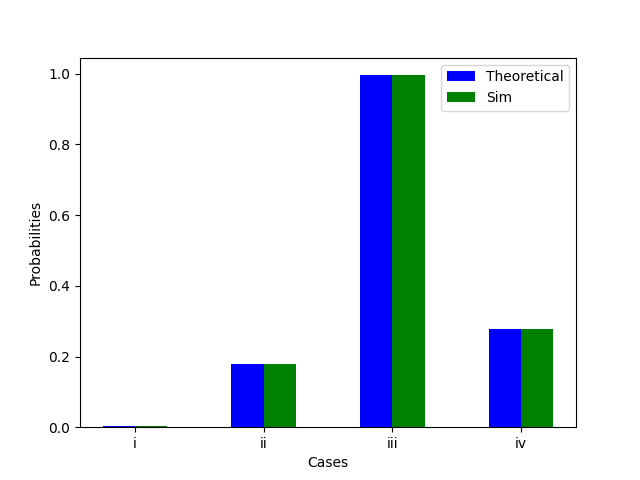
\includegraphics[width=0.45\textwidth]{Figure_1.png}
 
\end{document}